\documentclass[a4paper]{article}

% Basic packages
\usepackage[fontset=fandol]{ctex}
\usepackage{amsmath, amssymb}
\usepackage{graphicx}
\usepackage{xcolor}
\usepackage[margin=2.4cm]{geometry}
\usepackage{etoolbox}
\usepackage{listings}
\usepackage{hyperref}
\usepackage{xurl}
\usepackage{booktabs}
\usepackage{longtable}
\usepackage{tabularx}
\usepackage{array}
\usepackage{subcaption}
\usepackage{float}
\usepackage{enumitem}

\hypersetup{
    colorlinks=true,
    linkcolor=blue!50!black,
    urlcolor=blue!60!black,
    citecolor=blue!50!black
}

\definecolor{gray}{gray}{0.45}

\newenvironment{findingbox}[1]{\par\medskip\noindent\textbf{#1}\par\begin{quote}\itshape}{\end{quote}\medskip}
\newenvironment{evidencebox}[1]{\par\medskip\noindent\textbf{#1}\par\begin{quote}}{\end{quote}\medskip}
\newenvironment{riskbox}[1]{\par\medskip\noindent\textbf{#1}\par\begin{quote}}{\end{quote}\medskip}
\newenvironment{methodbox}[1]{\par\medskip\noindent\textbf{#1}\par\begin{quote}}{\end{quote}\medskip}

\lstset{
    language=Python,
    basicstyle=\ttfamily\small,
    keywordstyle=\color{blue},
    stringstyle=\color{red!60!black},
    commentstyle=\color{green!50!black},
    breaklines=true,
    frame=single,
    numbers=left,
    numberstyle=\tiny\color{gray},
    captionpos=b,
    extendedchars=false
}

\newcolumntype{Y}{>{\raggedright\arraybackslash}X}
\setlist[itemize]{leftmargin=1.8em}
\setlength{\LTleft}{0pt}
\setlength{\LTright}{0pt}

\newcommand{\reporttitle}{GenRec Instruments-grec RL 实验深度复盘}
\newcommand{\reportsubtitle}{Reward Form、Hint Scaffold 与 Offline/Online Gap 的代码对照分析}
\newcommand{\reportauthors}{Codex}
\newcommand{\reportdate}{2026-03-28}
\newcommand{\researchquestion}{在当前 Instruments-grec 结果上，哪些 RL 设计真正有效，当前最可信的 contribution 是什么，以及为什么离线 hint 结果显著好于在线最终评测？}
\newcommand{\reportscope}{覆盖 20 个用户指定结果目录、SFT 基线、离线 beam16 hint bundle、以及当前仓库相关训练与评测代码；证据截止到 2026-03-28 本地仓库快照。}
\newcommand{\reportaudience}{GenRec 内部研究与实验推进者，目标是决定 paper framing、主打实验和下一轮 ablation。}
\newcommand{\sourcewindow}{本地结果与代码访问日期：2026-03-28}
\newcommand{\reportcoverpath}{figures/hint_tradeoff_scatter.png}

\begin{document}

\begin{titlepage}
\centering
{\Large 深度研究报告\par}
\vspace{1.0cm}
{\huge\bfseries \reporttitle\par}
\vspace{0.5cm}
{\Large \reportsubtitle\par}
\vspace{0.9cm}
{\large \reportauthors\par}
\vspace{0.2cm}
{\large \reportdate\par}
\vspace{1.0cm}

\includegraphics[width=0.84\textwidth,height=0.42\textheight,keepaspectratio]{\reportcoverpath}\par

\vfill
\fbox{\parbox{0.94\textwidth}{
\textbf{核心问题}：\researchquestion\par
\textbf{研究范围}：\reportscope\par
\textbf{目标读者}：\reportaudience\par
\textbf{证据窗口}：\sourcewindow\par
}}
\end{titlepage}

\tableofcontents
\newpage

\section{执行摘要}

\begin{findingbox}{一句话结论}
当前最可信、也最值得写成主线 contribution 的结论不是“复杂 reward shaping”，而是“\textbf{task-aware oracle scaffold 能比复杂 reward 形状更稳定地缓解 semantic-ID RL 的稀疏性}”。在现有结果里，\textbf{fixed hint + rule-only} 是最平衡的方向：它几乎追平最强 top-10 指标，同时显著修复了 plain rule-only 的 top-50 coverage 损失。
\end{findingbox}

\begin{itemize}
\item 无 hint 的 reward form 对比里，best \texttt{NDCG@10} 仍然来自 \textbf{rule-only rerun}：\texttt{0.0960}；它比 baseline mixed GRPO 高 \texttt{+0.0008}，比 \texttt{prefix only} 高 \texttt{+0.0098}，说明 exact reward 在当前设定下并没有像直觉上那样拖垮 top-10。
\item 但 plain rule-only 的代价是 coverage 收缩：best \texttt{HR@50=0.1681}，低于 SFT 基线的 \texttt{0.1844}；这个结构性问题在 mixed GRPO 上也存在。
\item \textbf{fixed hint mixed-single} 的 best 点达到 \texttt{NDCG@10=0.0953}、\texttt{HR@10=0.1193}、\texttt{NDCG@50=0.1114}、\texttt{HR@50=0.1938}。相对 plain rule-only，它只损失 \texttt{0.0007} 的 \texttt{NDCG@10}，却换来 \texttt{+0.0257} 的 \texttt{HR@50} 增益。
\item reward shaping 不是完全没用，但高度依赖 credit assignment 细节。最明显的证据是 \texttt{prefix tokenadv raw} 几乎崩掉，而加上 \texttt{totalnorm} 后 \texttt{NDCG@10} 直接回升 \texttt{+0.0430}。
\item fixed 当前赢 dynamic，核心更像是“\textbf{稳定但略偏的 scaffold}”打赢了“\textbf{自适应但由 one-hit-any 门控驱动的抖动 scaffold}”，而不是 dynamic 这个方向在理论上更差。
\item “ranking 好像不加比较好”这件事，当前证据支持“\textbf{至少没有显示出明确收益}”。在 dynamic hint 组里，\texttt{ranking} 版本四个主指标都弱于 \texttt{rule-only + gather fix}。代码层面也能解释：ranking reward 只有在 group 内已经出现 exact hit 时才会激活，它对最难的“全组 0 hit”样本几乎没有帮助。
\end{itemize}

\section{研究范围与方法}

\begin{methodbox}{证据清单与口径}
本报告使用四类主证据：
\begin{itemize}
\item \textbf{S1}: 用户指定的 20 个结果目录及其 \texttt{checkpoint-*/metrics.json}，另补 SFT 基线 \texttt{results/Instruments-grec-sft-qwen4B-4-256-dsz0/checkpoint-495/metrics.json}。
\item \textbf{S2--S4}: 本地 beam16 hint bundle，包括 \texttt{instruments\_grec\_beam16\_hint\_difficulty\_table.csv}、cascade summary 和 task-aware fixed hint map。
\item \textbf{S5--S9}: 当前仓库代码，重点是 \texttt{rewards/ranking\_reward.py}、\texttt{token\_prefix\_grpo\_trainer.py}、\texttt{trl\_trainer.py}、\texttt{fixed\_hint\_grpo\_trainer.py} 与 \texttt{evaluate.py}。
\item \textbf{S10--S12}: 仓库内先前分析文档，仅作为辅助语境，不作为唯一证据来源。
\end{itemize}
\end{methodbox}

本文所有“best checkpoint”默认按 \texttt{NDCG@10} 选点。相对 SFT 的相对增益定义为：
$$
\Delta_{\mathrm{rel}}(m)=\frac{m_{\mathrm{variant}}-m_{\mathrm{SFT}}}{m_{\mathrm{SFT}}}
$$
\begin{itemize}
\item $m_{\mathrm{variant}}$：某个 RL 变体在其 best checkpoint 上的指标
\item $m_{\mathrm{SFT}}$：SFT 基线 \texttt{checkpoint-495} 上的同名指标
\item $\Delta_{\mathrm{rel}}(m)$：相对提升或相对下降比例
\end{itemize}

本报告还对用户点名的全部目录做了分类：
\begin{itemize}
\item \textbf{主结论 run}: 当前可稳定解释、脚本与结果目录对应明确的 reward/hint ablation。
\item \textbf{superseded/legacy run}: 旧 run、明显异常 run、仅单 checkpoint backup，保留作排错和演化证据，不拿来做主结论。
\item \textbf{代码证据}: 用于解释 reward 定义、hint 何时参与训练/评测、以及 dynamic/fixed hint 的真正行为。
\end{itemize}

\section{实验版图与目录口径}

用户给的目录并不是一个完全同质的 ablation matrix，而是混合了三类东西：
\begin{itemize}
\item 同一想法的 \textbf{旧名/旧 run}，例如 \texttt{prefix} old alias 与后续 \texttt{prefixonly-ndcg-rule0}。
\item \textbf{修复后 rerun}，例如 \texttt{rule-only-rerun-quietlog}、\texttt{prefix-seq-only-fixbool-rerun}。
\item \textbf{真正新的方法线}，例如 dynamic hint、fixed hint、task-aware fixed hint、sid-only dynamic hint。
\end{itemize}

因此，合理的阅读方式不是把 20 个目录一视同仁，而是先明确主比较轴：
\begin{itemize}
\item \textbf{Reward form 主轴}：baseline mixed GRPO、rule-only、prefix only、prefix seq only、prefix token only、tokenadv raw、tokenadv totalnorm、tokenadv errtok。
\item \textbf{Hint 主轴}：plain rule-only、dynamic hint rule-only、dynamic hint + ranking、dynamic hint sid-only、fixed hint mixed-single、fixed hint taskfix。
\item \textbf{历史/排错证据}：old rule-only、old prefix-seq-only、prefix backup、single-checkpoint backup、早期 task-index fix run。
\end{itemize}

\begin{riskbox}{哪些 run 不该当主结论}
\texttt{Instruments-grec-grpo-rule-only-qwen...} 和 \texttt{Instruments-grec-grpo-prefix-seq-only-qwen...} 与对应 rerun 的差距极大，说明旧 run 至少混入了实现或配置问题；它们更适合证明“修复有用”，不适合证明“方法本身差”。相反，\texttt{prefix} old alias 与正式 \texttt{prefixonly-ndcg-rule0} 几乎重合，更像命名演化而不是方法差异。
\end{riskbox}

\subsection{版本时间线与 bug 对齐}

把结果目录和脚本历史对上以后，这批实验其实分成三个阶段：
\begin{itemize}
\item \textbf{2026-03-17 之前后}: 旧版 dynamic 与旧版 fixed。对应目录分别是 \texttt{...dynamic-hint-cascade...} 和 \texttt{...fixed-hint-mixed-single-generate...}。这时 fixed hint map 仍按 \texttt{extra\_info.index} 导出，dynamic trainer 也还没有后来的 gather 修复。
\item \textbf{2026-03-20}: commit ``Fix hint training map export and launch defaults'' 同时修了两件事。第一，fixed hint export 从 \texttt{index} 升级为 \texttt{task+index}；第二，dynamic trainer 加入了跨 rank unresolved-group 同步与 pure rule-only 的 selected-rule-reward gather fast path。修复后默认目录变成 \texttt{...fixedhint-taskfix-b16-sft495} 和 \texttt{...dynamic-hint-cascade-reward-gather-fix...}。
\item \textbf{2026-03-28}: 新增 \texttt{ranking dynamic hint} 与 \texttt{sid-only dynamic hint} 脚本。这一点很重要，因为它说明 ranking dynamic 不是跑在“旧 dynamic bug 版”上的，而是跑在 3 月 20 日修复之后的 dynamic trainer 上。
\end{itemize}

因此，后文里涉及 dynamic 的主结论都应该优先使用 \texttt{reward-gather-fix} 版本；涉及 fixed 的主结论则必须明确区分“旧 index-only hint map”与“修复后的 task+index hint map”。

\section{主结果一：Reward Form Ablation}

SFT 基线为：\texttt{NDCG@10=0.0823}、\texttt{HR@10=0.1094}、\texttt{NDCG@50=0.0985}、\texttt{HR@50=0.1844}。

\begin{table}[H]
\centering
\small
\begin{tabular}{p{4.0cm}p{1.7cm}cccc}
\toprule
Variant & Best ckpt & NDCG@10 & HR@10 & NDCG@50 & HR@50 \\
\midrule
Baseline mixed GRPO & checkpoint-1665 & 0.0952 & 0.1145 & 0.1071 & 0.1696 \\
Rule only rerun & checkpoint-2997 & 0.0960 & 0.1179 & 0.1070 & 0.1681 \\
Prefix only & checkpoint-1332 & 0.0862 & 0.1049 & 0.0982 & 0.1612 \\
Prefix seq only rerun & checkpoint-1332 & 0.0857 & 0.1046 & 0.0985 & 0.1636 \\
Prefix token only & checkpoint-1665 & 0.0815 & 0.1005 & 0.0958 & 0.1668 \\
Prefix tokenadv raw & checkpoint-999 & 0.0476 & 0.0597 & 0.0564 & 0.0991 \\
Prefix tokenadv totalnorm & checkpoint-3326 & 0.0906 & 0.1125 & 0.1054 & 0.1809 \\
Prefix tokenadv errtok & checkpoint-999 & 0.0796 & 0.0968 & 0.0914 & 0.1513 \\
\bottomrule
\end{tabular}
\caption{Reward form 主结果表。来源：S1，按 best \texttt{NDCG@10} 选点。}
\end{table}

\begin{figure}[H]
\centering
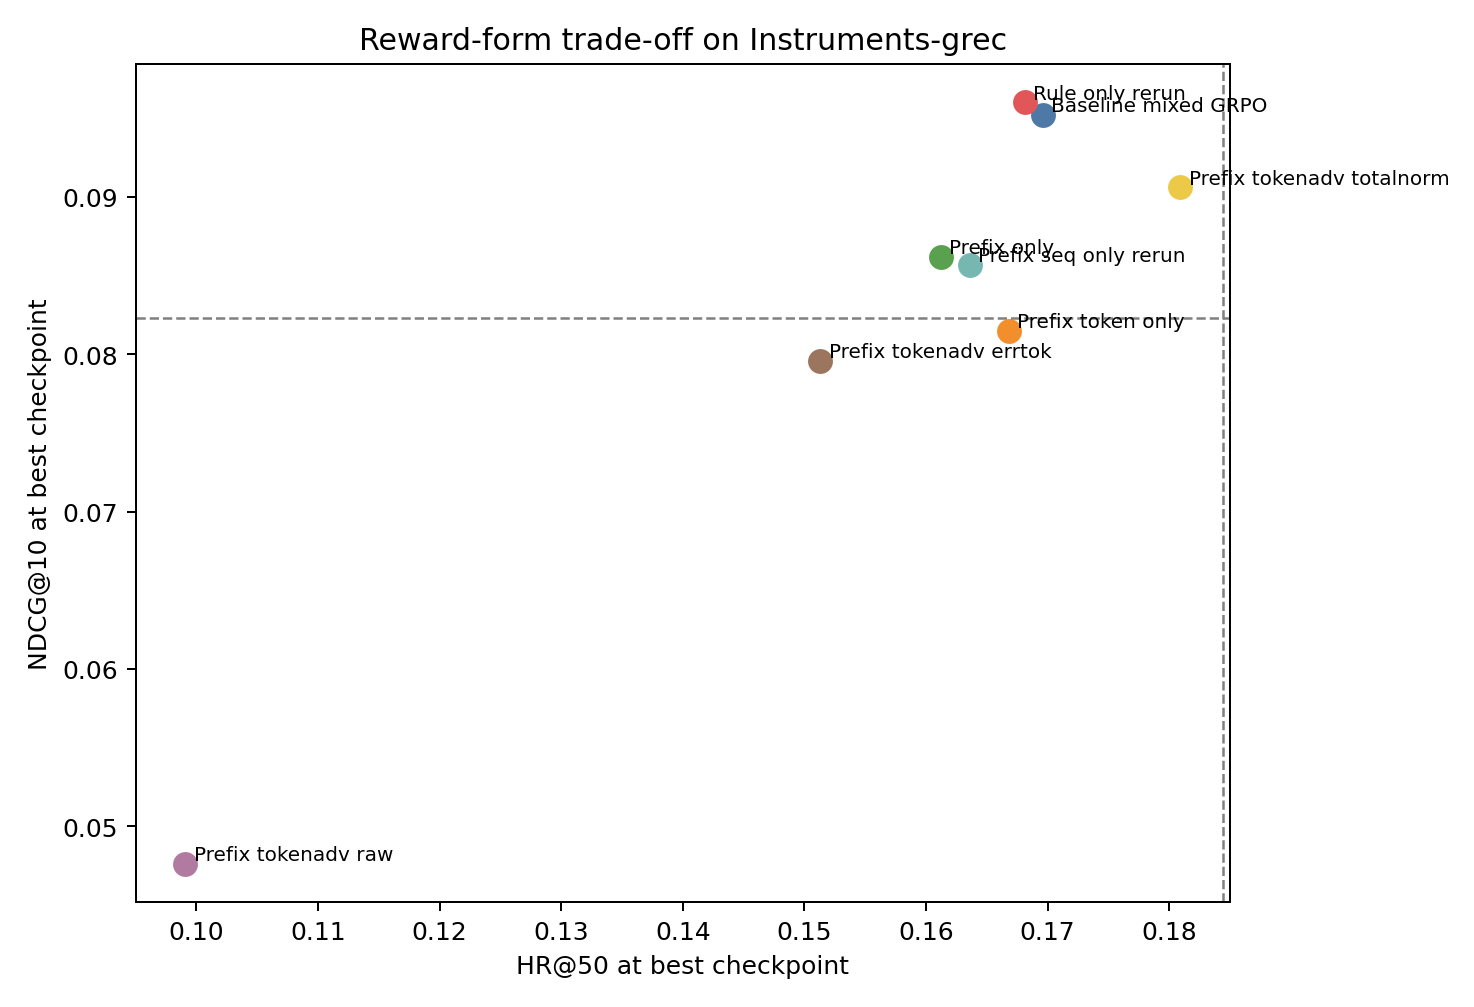
\includegraphics[width=0.86\textwidth]{figures/reward_tradeoff_scatter.png}
\caption{Reward 形式在 top-10 与 top-50 coverage 上的 trade-off。}
\end{figure}
\footnotetext{来源：作者基于 \texttt{docs/deepresearch/genrec\_rl\_study\_2026-03-28/data/experiment\_best\_metrics.csv} 自绘；底层数据来自 \texttt{results/*/checkpoint-*/metrics.json}。}

\subsection{rule-only 仍然是当前最强的无 hint top-10 基线}

最强的无 hint top-10 指标来自 \textbf{rule-only rerun} 而不是更复杂的 shaping：
\begin{itemize}
\item \texttt{rule-only rerun}: \texttt{NDCG@10=0.0960}, \texttt{HR@10=0.1179}
\item baseline mixed GRPO: \texttt{NDCG@10=0.0952}, \texttt{HR@10=0.1145}
\end{itemize}

二者差异不大，但方向很清楚：相较 baseline mixed GRPO，rule-only 在 \texttt{NDCG@10} 上仍有 \texttt{+0.0008} 的优势，在 \texttt{HR@10} 上有 \texttt{+0.0034} 的优势。这说明当前任务最核心的矛盾并不是“exact reward 太 sparse 所以一定打不过 dense reward”，而是“dense reward 是否真的对 hardest case 提供了有用的信用分配”。

\subsection{纯 prefix reward 不能替代 exact reward}

\texttt{prefix only} 和 \texttt{prefix seq only rerun} 的表现都明显弱于 rule-only：
\begin{itemize}
\item \texttt{prefix only}: \texttt{NDCG@10=0.0862}
\item \texttt{prefix seq only rerun}: \texttt{NDCG@10=0.0857}
\item \texttt{rule-only rerun}: \texttt{NDCG@10=0.0960}
\end{itemize}

绝对差距分别是 \texttt{0.0098} 和 \texttt{0.0103}。这不是噪声量级，说明“只鼓励前缀更长”并不足以支撑最后的 next-item 排序质量。结合离线 hint bundle 的结论，更合理的解释是：
\begin{itemize}
\item 前两位 SID token 确实决定了大多数样本的难度分层；
\item 但训练目标如果只奖励 prefix，而不继续对最终 exact item 负责，就会把“会走到正确 bucket”和“能完成最终辨识”混在一起。
\end{itemize}

\subsection{token-level prefix advantage 不是不能用，但必须处理归一化}

最强的工程信号来自 \texttt{tokenadv raw} 与 \texttt{tokenadv totalnorm} 的对比：
\begin{itemize}
\item \texttt{prefix tokenadv raw}: \texttt{NDCG@10=0.0476}, \texttt{HR@50=0.0991}
\item \texttt{prefix tokenadv totalnorm}: \texttt{NDCG@10=0.0906}, \texttt{HR@50=0.1809}
\end{itemize}

也就是说，只改一层 total-token normalization，就带来：
\begin{itemize}
\item \texttt{NDCG@10 +0.0430}
\item \texttt{HR@10 +0.0528}
\item \texttt{NDCG@50 +0.0490}
\item \texttt{HR@50 +0.0818}
\end{itemize}

这不是“微调 credit assignment 会有一点提升”，而是“\textbf{不做对的 normalization 会直接把训练打坏}”。

\subsection{errtok 版本目前没有带来额外收益}

\texttt{prefix tokenadv totalnorm errtok} 的出发点是合理的：不要把负信号打到已经正确的 prefix token 上，只惩罚错误 token 及其后缀。但现有结果并不支持它优于普通 totalnorm：
\begin{itemize}
\item 相比 \texttt{totalnorm}，\texttt{errtok} 在 \texttt{NDCG@10} 上低 \texttt{0.0110}
\item 在 \texttt{HR@50} 上低 \texttt{0.0296}
\end{itemize}

这说明“错误 token 专属惩罚”这个想法本身未必错，但当前实现、权重比例或归一化方式还没有对齐任务主矛盾。

\subsection{reward 线的可信结论}

\begin{findingbox}{Reward 线现在可以站得住的结论}
\begin{itemize}
\item 当前最强的无 hint top-10 baseline 仍然是 \textbf{rule-only rerun}。
\item 纯 prefix reward 不能替代 exact reward，只能视作辅助信号候选。
\item token-level prefix reward 想要可用，关键不在“更细粒度”本身，而在 \textbf{normalization 与 credit assignment 是否稳定}。
\end{itemize}
\end{findingbox}

\section{主结果二：Hint Scaffold Ablation}

\begin{table}[H]
\centering
\small
\begin{tabular}{p{4.5cm}p{1.7cm}cccc}
\toprule
Variant & Best ckpt & NDCG@10 & HR@10 & NDCG@50 & HR@50 \\
\midrule
Dynamic hint + ranking & checkpoint-1665 & 0.0911 & 0.1138 & 0.1058 & 0.1822 \\
Dynamic hint rule-only (old) & checkpoint-1665 & 0.0919 & 0.1160 & 0.1080 & 0.1905 \\
Dynamic hint rule-only + gather fix & checkpoint-2997 & 0.0936 & 0.1169 & 0.1083 & 0.1855 \\
Dynamic hint sid-only & checkpoint-2394 & 0.0921 & 0.1155 & 0.1065 & 0.1830 \\
Fixed hint mixed-single & checkpoint-3326 & 0.0953 & 0.1193 & 0.1114 & 0.1938 \\
Fixed hint task+index early & checkpoint-666 & 0.0894 & 0.1131 & 0.1051 & 0.1864 \\
Fixed hint taskfix b16 & checkpoint-2997 & 0.0931 & 0.1189 & 0.1094 & 0.1941 \\
\bottomrule
\end{tabular}
\caption{Hint 主结果表。来源：S1，按 best \texttt{NDCG@10} 选点。}
\end{table}

\begin{figure}[H]
\centering
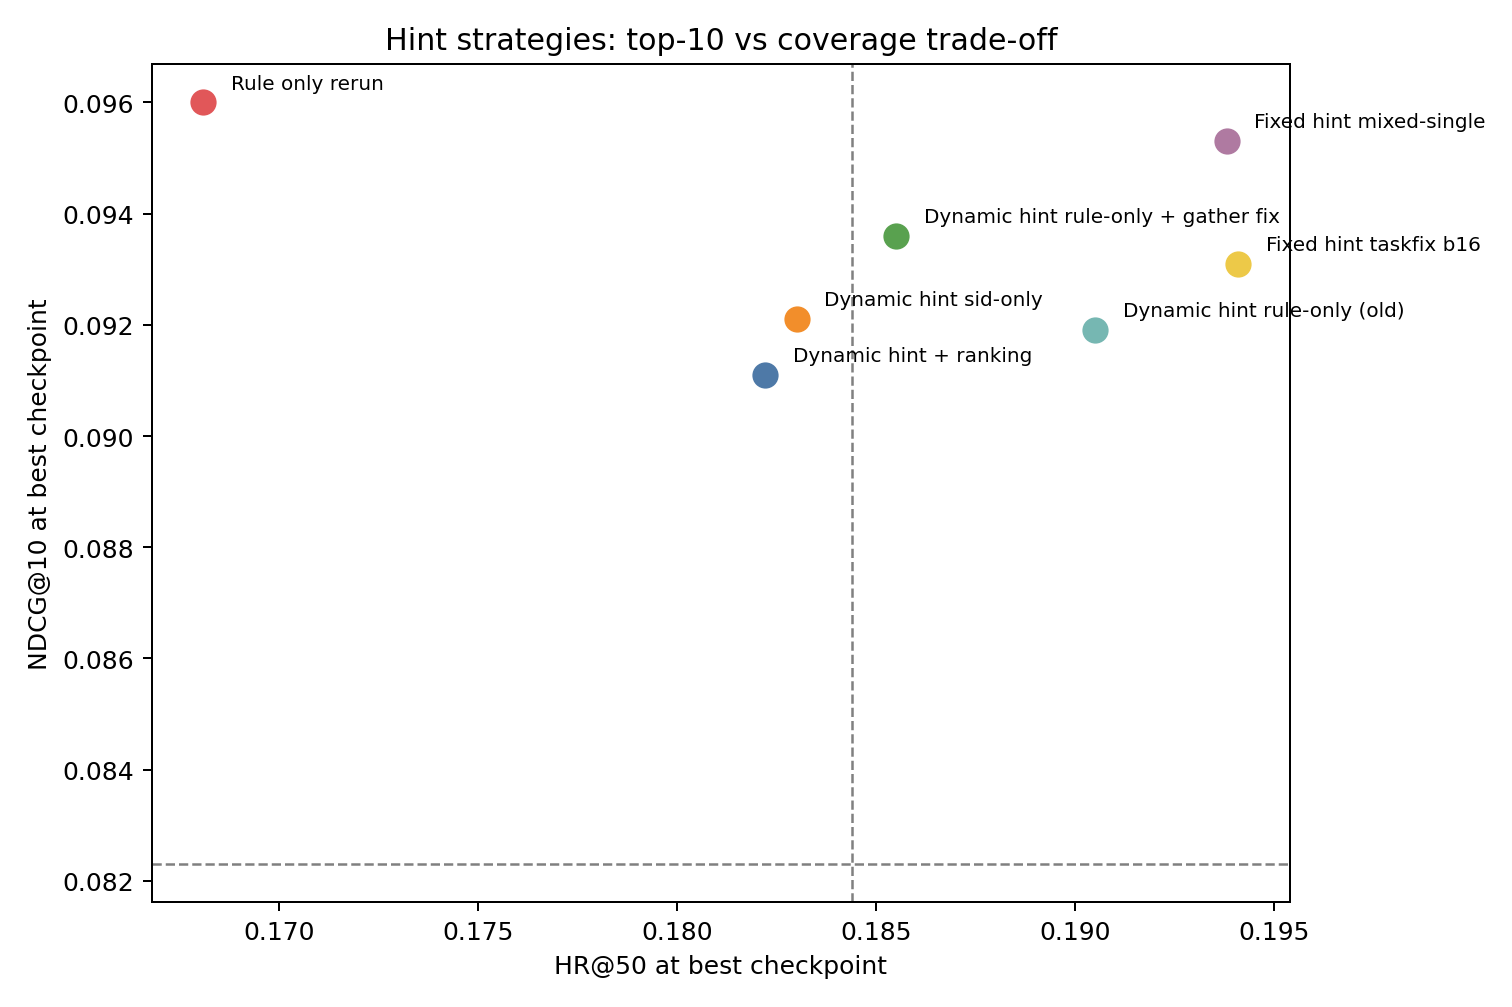
\includegraphics[width=0.86\textwidth]{figures/hint_tradeoff_scatter.png}
\caption{Hint 方案的 top-10 / coverage trade-off。}
\end{figure}
\footnotetext{来源：作者基于 \texttt{experiment\_best\_metrics.csv} 自绘。}

\begin{figure}[H]
\centering
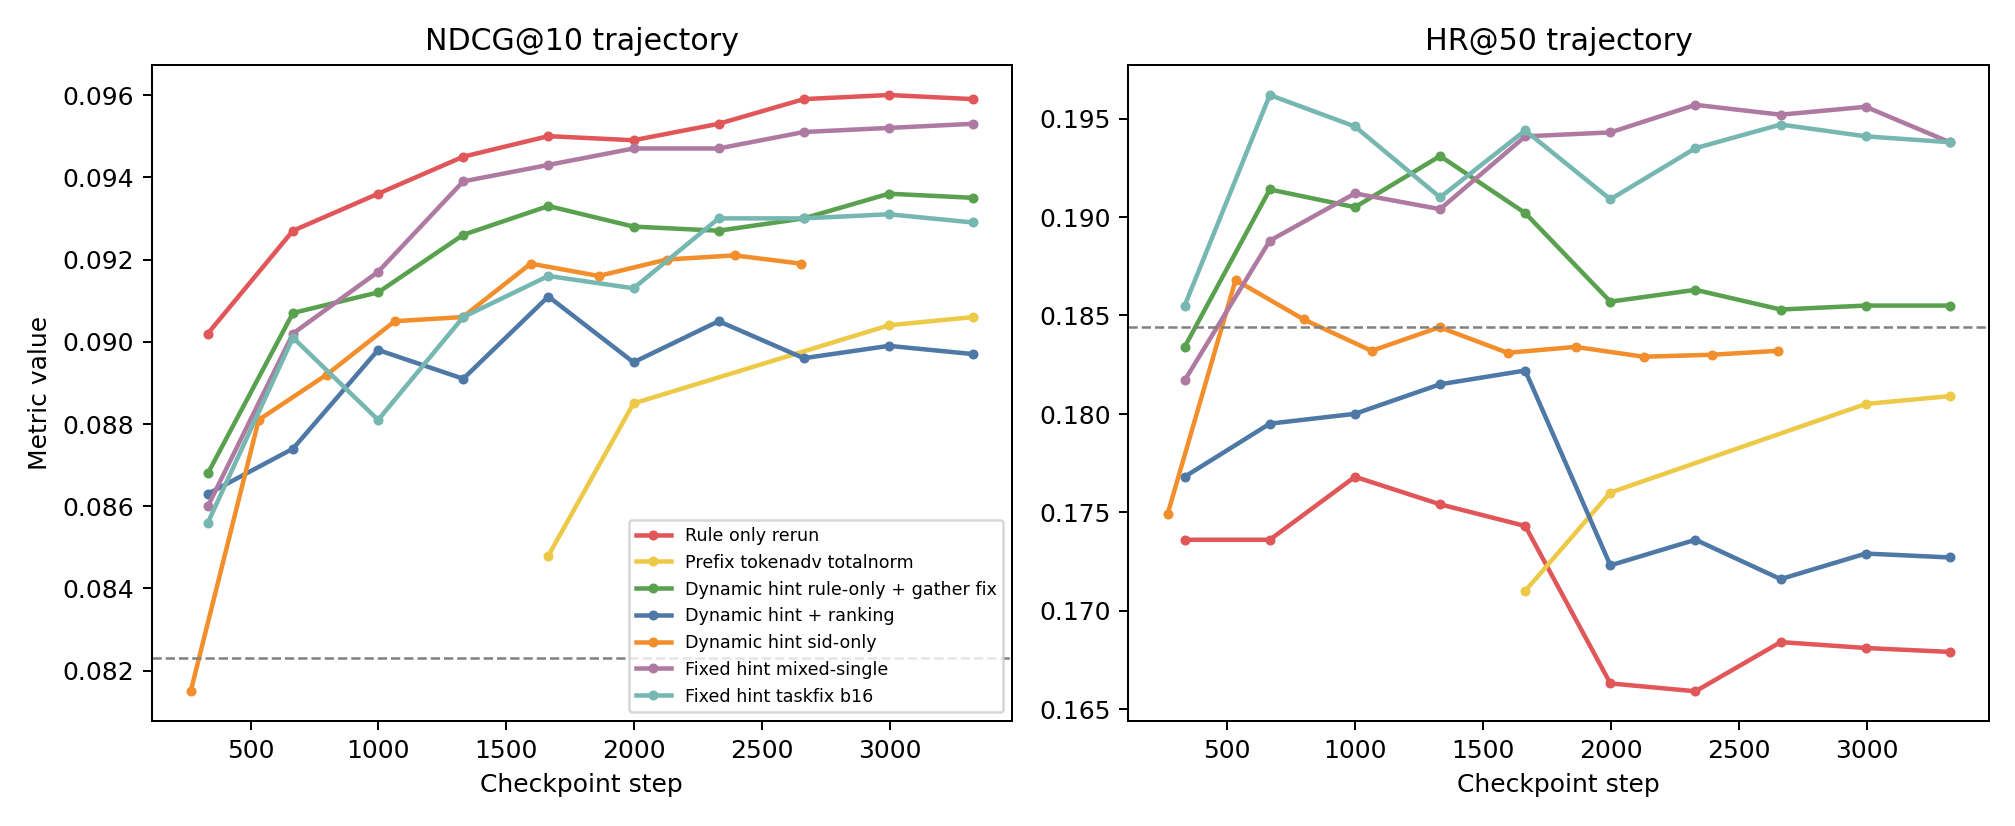
\includegraphics[width=\textwidth]{figures/selected_trajectories.png}
\caption{代表性实验的训练轨迹。左图为 \texttt{NDCG@10}，右图为 \texttt{HR@50}。}
\end{figure}
\footnotetext{来源：作者基于 \texttt{metrics.json} 时间序列自绘。灰色虚线为 SFT 基线。}

\subsection{fixed hint 是当前最平衡、也最值得写成主结果的方向}

如果只看 best \texttt{NDCG@10}，plain rule-only 仍然略高于 fixed hint mixed-single：
\begin{itemize}
\item \texttt{rule-only rerun}: \texttt{NDCG@10=0.0960}
\item \texttt{fixed hint mixed-single}: \texttt{NDCG@10=0.0953}
\end{itemize}

但这个差距只有 \texttt{0.0007}，几乎可以理解成“固定 scaffold 没有牺牲 top-10”。与此同时，fixed hint mixed-single 带来了明显更强的 coverage：
\begin{itemize}
\item \texttt{NDCG@50 +0.0044} relative to plain rule-only
\item \texttt{HR@50 +0.0257} relative to plain rule-only
\end{itemize}

这条结果很关键，因为它说明 fixed hint 不是“靠 hint 把 top-10 做差了但 coverage 变好”，而是“\textbf{几乎保住 top-10，同时显著修复 coverage}”。

\subsection{task-aware fixed hint map 更安全，且仍然保住了 coverage}

\texttt{fixed hint taskfix b16} 是更值得信的工程版本，因为它对齐了 \texttt{task+index} 复合 sample key，而不是单独使用 \texttt{index}。这条线的 best 点是：
\begin{itemize}
\item \texttt{NDCG@10=0.0931}
\item \texttt{HR@50=0.1941}
\end{itemize}

和旧的 fixed hint mixed-single 相比：
\begin{itemize}
\item \texttt{NDCG@10} 低 \texttt{0.0022}
\item \texttt{HR@50} 高 \texttt{0.0003}
\end{itemize}

这里真正被修掉的不是“泄漏”，而是 \textbf{cross-task index collision}。相同 \texttt{index} 在不同 task 上可能对应不同最小有效 hint depth；旧版 index-only map 会把它们错误地折叠成一个共享 depth。

\subsection{旧 fixed 错版为什么反而更好：它本质上是一个更浅的 hint curriculum}

\begin{figure}[H]
\centering
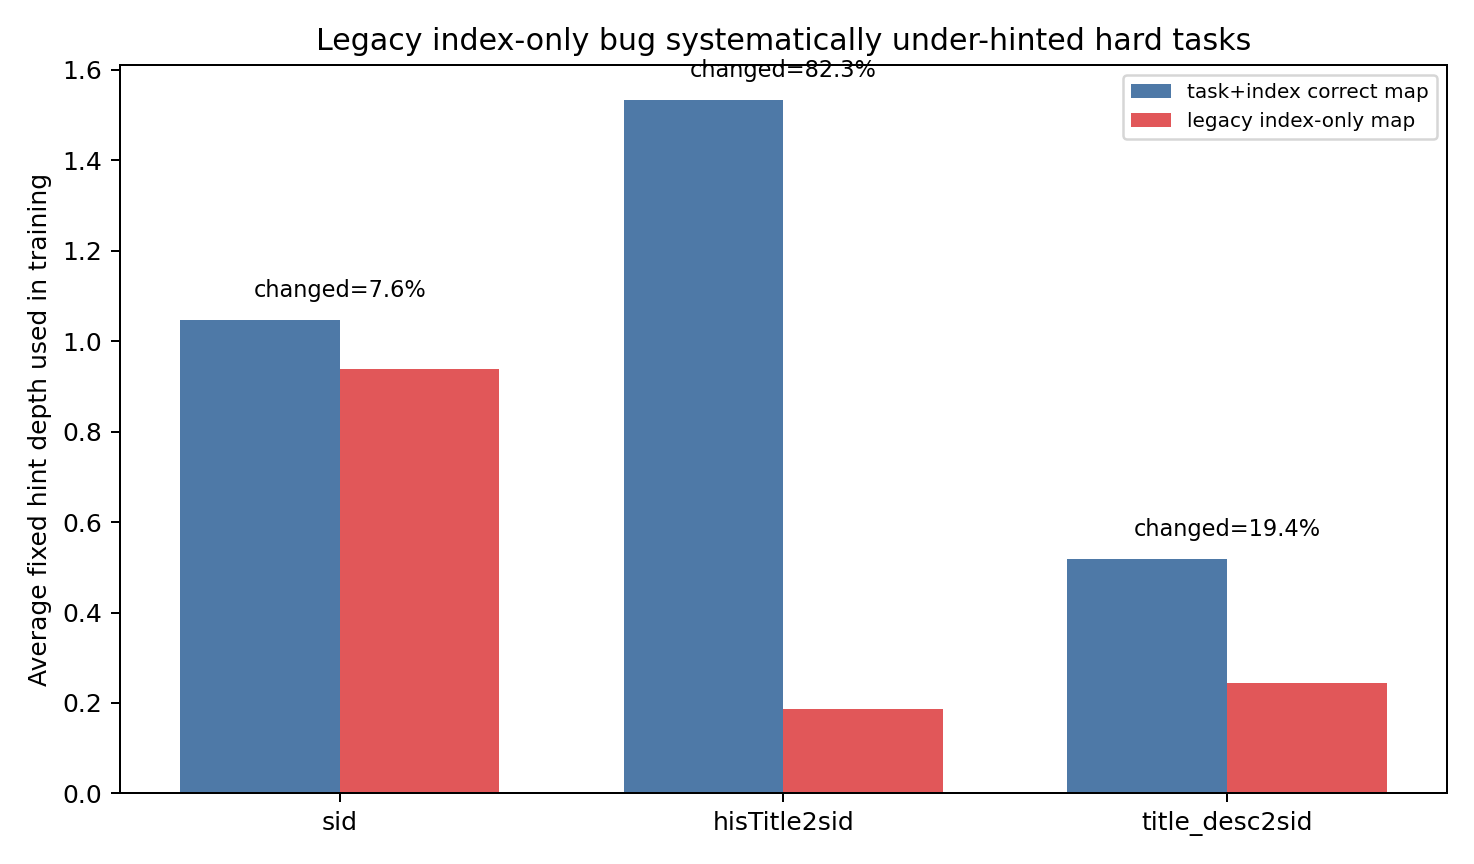
\includegraphics[width=0.82\textwidth]{figures/fixed_hint_bug_depth_shift.png}
\caption{旧的 index-only fixed hint bug 会系统性压浅 hard task 的 hint 深度。}
\end{figure}
\footnotetext{来源：作者基于 \texttt{instruments\_grec\_beam16\_hint\_difficulty\_table.csv} 重建“legacy index-only map”与“task+index correct map”后自绘。}

\begin{figure}[H]
\centering
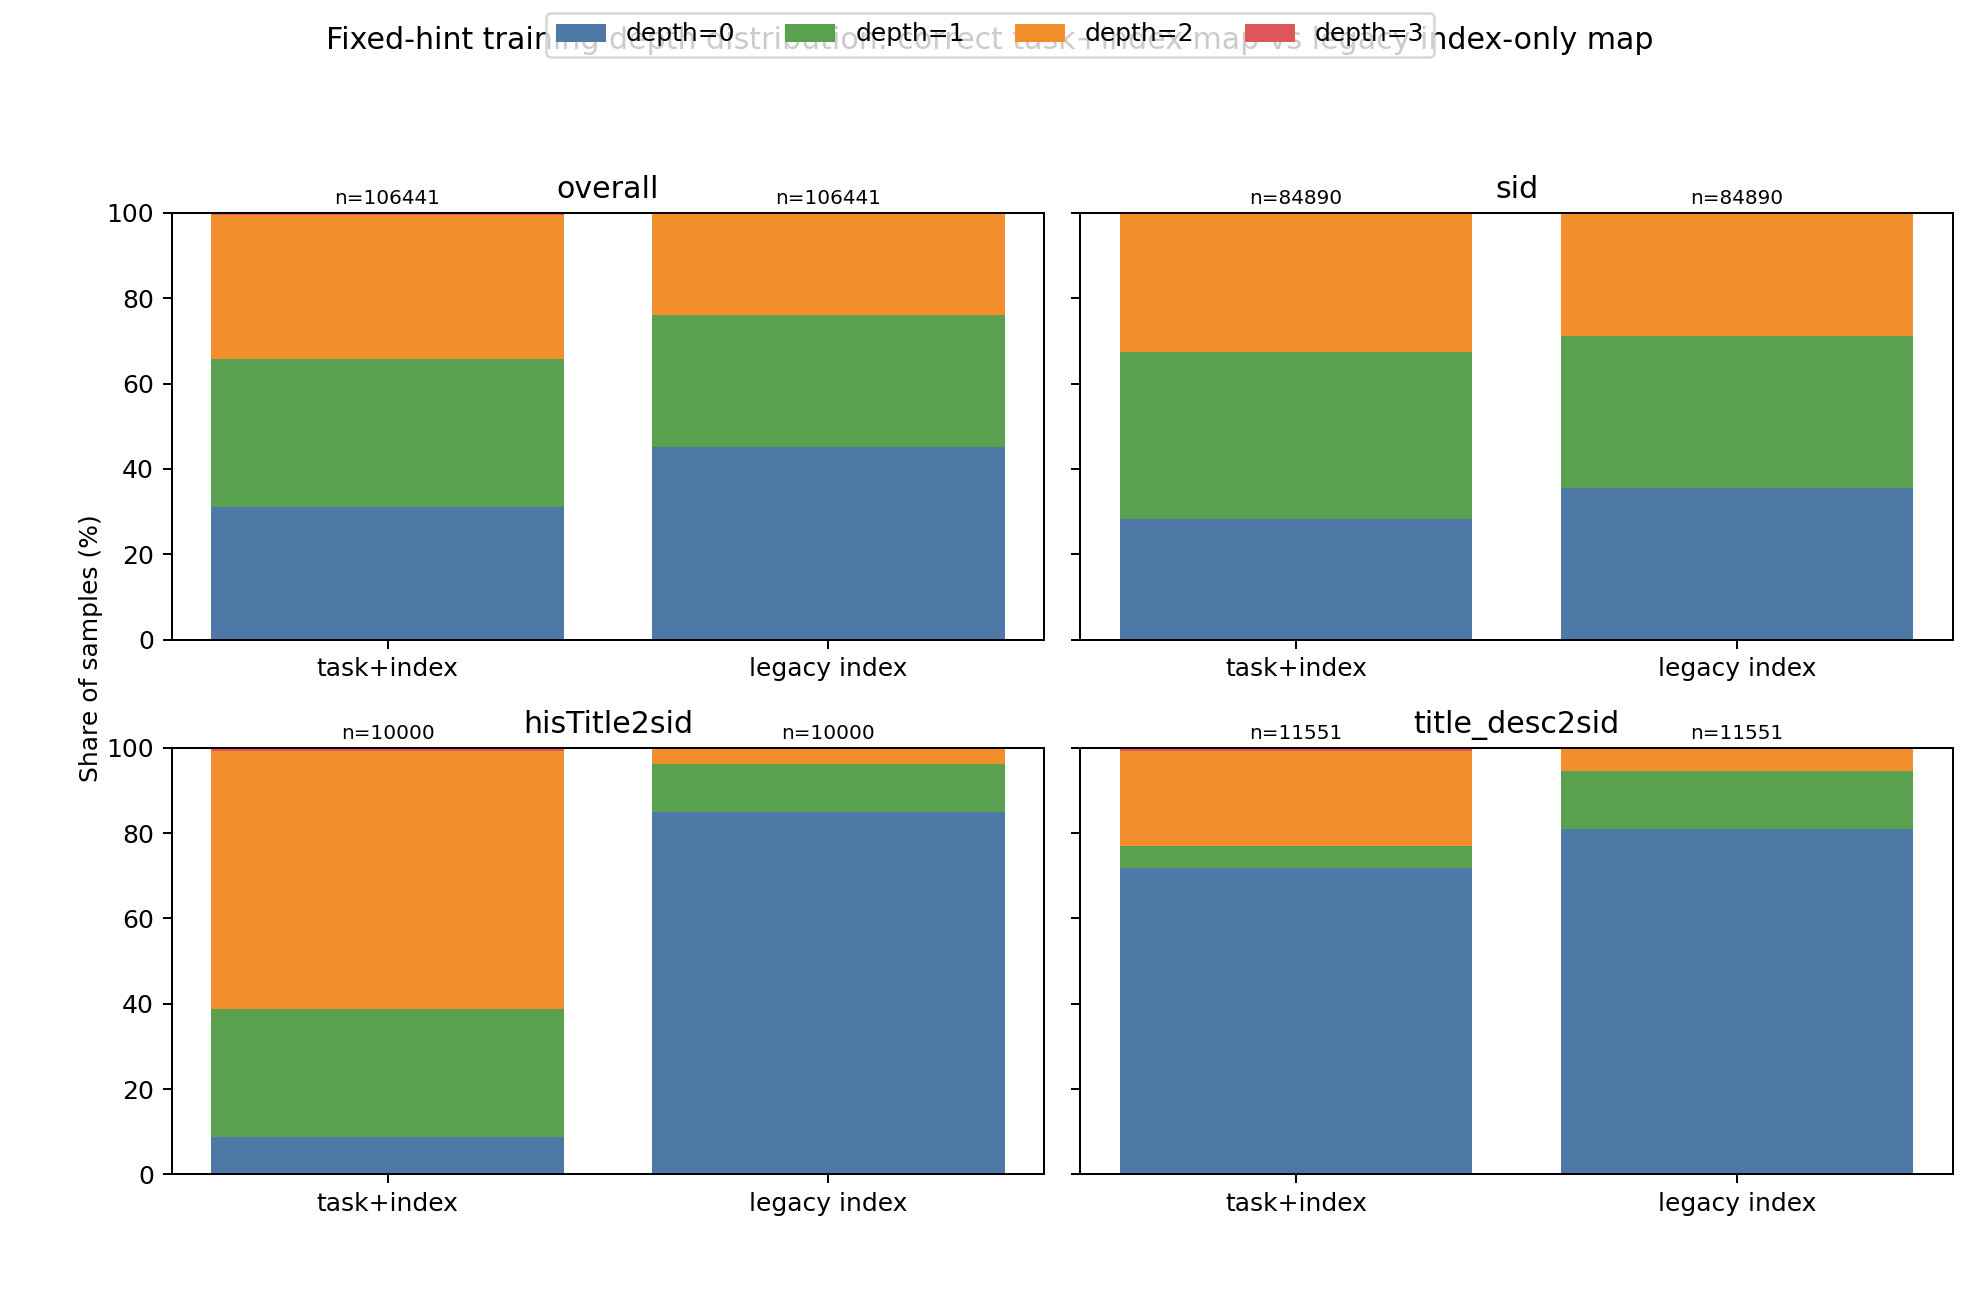
\includegraphics[width=0.94\textwidth]{figures/fixed_hint_bug_depth_distribution.png}
\caption{旧 fixed bug 与修复后 fixed 在 overall 及各 task 上的 hint-depth 分布。}
\end{figure}
\footnotetext{来源：作者基于 \texttt{fixed\_hint\_bug\_depth\_distribution.csv} 自绘。}

\begin{table}[H]
\centering
\small
\begin{tabular}{p{2.5cm}p{2.2cm}cccc}
\toprule
Scope & Version & depth=0 & depth=1 & depth=2 & depth=3 \\
\midrule
overall & task+index & 31.1\% & 34.5\% & 33.9\% & 0.4\% \\
overall & legacy index & 45.0\% & 30.9\% & 23.8\% & 0.2\% \\
sid & task+index & 28.3\% & 39.0\% & 32.4\% & 0.3\% \\
sid & legacy index & 35.4\% & 35.6\% & 28.7\% & 0.3\% \\
hisTitle2sid & task+index & 8.7\% & 30.1\% & 60.5\% & 0.8\% \\
hisTitle2sid & legacy index & 85.0\% & 11.2\% & 3.8\% & 0.0\% \\
title\_desc2sid & task+index & 71.8\% & 5.2\% & 22.2\% & 0.8\% \\
title\_desc2sid & legacy index & 80.9\% & 13.7\% & 5.4\% & 0.0\% \\
\bottomrule
\end{tabular}
\caption{旧 fixed bug 与修复后 fixed 的训练期 hint-depth 比例。来源：\texttt{fixed\_hint\_bug\_depth\_distribution.csv}。}
\end{table}

把离线难度表重新按“旧 bug 逻辑”折叠一遍后，可以看到这个 bug 不是轻微扰动，而是大幅改变了训练期 scaffold 强度：
\begin{itemize}
\item 全体样本里有 \texttt{15.94\%} 的 hint depth 被压浅。
\item 对 \texttt{sid}，变化率只有 \texttt{7.64\%}，平均深度从 \texttt{1.048} 降到 \texttt{0.938}。
\item 对 \texttt{title\_desc2sid}，变化率是 \texttt{19.41\%}，平均深度从 \texttt{0.519} 降到 \texttt{0.245}。
\item 对 \texttt{hisTitle2sid}，变化率高达 \texttt{82.35\%}，平均深度从 \texttt{1.533} 直接降到 \texttt{0.188}。
\end{itemize}

也就是说，旧 fixed 不是“hint 更准”，恰恰相反，它对 hardest task 大规模\textbf{少给了 hint}。仅 \texttt{hisTitle2sid} 一项里，就有：
\begin{itemize}
\item \texttt{2481} 个样本从 \texttt{1->0}
\item \texttt{5090} 个样本从 \texttt{2->0}
\item \texttt{586} 个样本从 \texttt{2->1}
\end{itemize}

如果直接看 hint 比例，这个 bug 的形状更明显：
\begin{itemize}
\item overall 上，旧版把 \texttt{depth=0} 比例从 \texttt{31.1\%} 抬到 \texttt{45.0\%}，同时把 \texttt{depth=2} 比例从 \texttt{33.9\%} 压到 \texttt{23.8\%}。
\item 对 \texttt{sid}，变化不算极端，但也把 \texttt{depth=0} 从 \texttt{28.3\%} 抬到了 \texttt{35.4\%}。
\item 对 \texttt{title\_desc2sid}，旧版把大量样本从 \texttt{depth=2} 挤到 \texttt{depth=1} 或 \texttt{depth=0}，\texttt{depth=2} 比例从 \texttt{22.2\%} 掉到 \texttt{5.4\%}。
\item 对 \texttt{hisTitle2sid}，旧版几乎把它整个“洗平”了：\texttt{depth=0} 直接从 \texttt{8.7\%} 暴涨到 \texttt{85.0\%}，\texttt{depth=2} 从 \texttt{60.5\%} 跌到 \texttt{3.8\%}。
\end{itemize}

这就给了“错版 fixed 反而更好”一个更可信的解释：旧 bug 意外形成了一个\textbf{更浅、更硬的 scaffold curriculum}。它让 hardest task 在训练时更接近 no-hint 条件，因此虽然优化更难，却可能更符合最终无 hint 评测的 transfer 目标。

这一点也能从逐 checkpoint 差值看出来：修复后的 \texttt{taskfix} 版本在很早期的 \texttt{HR@50} 往往不差，甚至在 \texttt{333/666/999} 这些点上略高；但从 \texttt{999} 之后开始，旧 fixed 在 \texttt{NDCG@10} 上几乎持续领先 \texttt{0.0017--0.0034}。更像是：
\begin{itemize}
\item 更深、更准确的 hint 让训练更容易；
\item 但也让训练目标离最终 no-hint eval 更远。
\end{itemize}

\subsection{dynamic hint 有价值，但 canonical 版本应以 gather-fix 为准}

dynamic hint line 的可信结论分三层：
\begin{itemize}
\item \textbf{第一层}: 旧 dynamic 结果已经被 3 月 20 日的 gather fix supersede，不应再作为 canonical baseline。
\item 它\textbf{确实能把 coverage 拉回到高于 SFT 的区间}，plain rule-only 做不到这一点。
\item 但它在当前结果里\textbf{仍然没有超过 fixed hint}。
\end{itemize}

\begin{figure}[H]
\centering
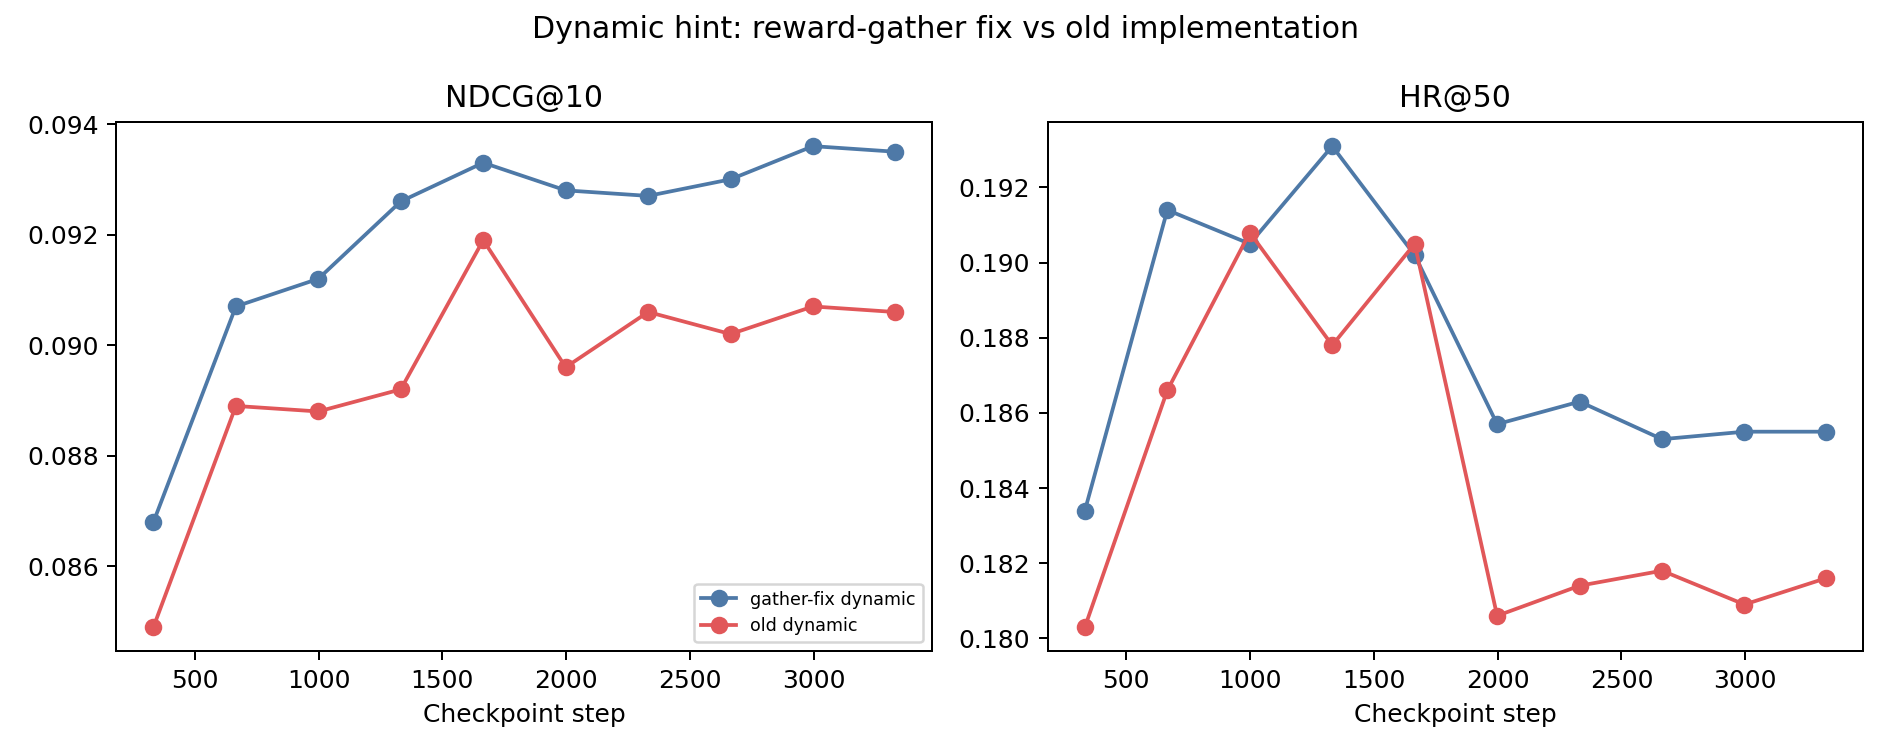
\includegraphics[width=\textwidth]{figures/dynamic_gather_fix_vs_old.png}
\caption{dynamic hint 的 gather-fix 版本在全部对齐 checkpoint 上都优于旧版本。}
\end{figure}
\footnotetext{来源：作者基于 \texttt{metrics\_inventory.csv} 中两条 dynamic run 的对齐 checkpoint 自绘。}

旧 dynamic 与 gather-fix dynamic 的逐 checkpoint 对比非常干净：在全部 \texttt{333--3326} 对齐 checkpoint 上，\texttt{gather-fix} 版本的 \texttt{NDCG@10} 都更高，提升区间是 \texttt{+0.0014} 到 \texttt{+0.0034}；\texttt{HR@10} 也全部更高，提升区间是 \texttt{+0.0006} 到 \texttt{+0.0048}。这说明 dynamic 旧版确实低估了 dynamic 路线本身的上限。

最好的 dynamic hint rule-only + gather fix 达到：
\begin{itemize}
\item \texttt{NDCG@10=0.0936}
\item \texttt{HR@50=0.1855}
\end{itemize}

相比 fixed hint mixed-single：
\begin{itemize}
\item \texttt{NDCG@10} 低 \texttt{0.0017}
\item \texttt{HR@50} 低 \texttt{0.0083}
\end{itemize}

\begin{figure}[H]
\centering
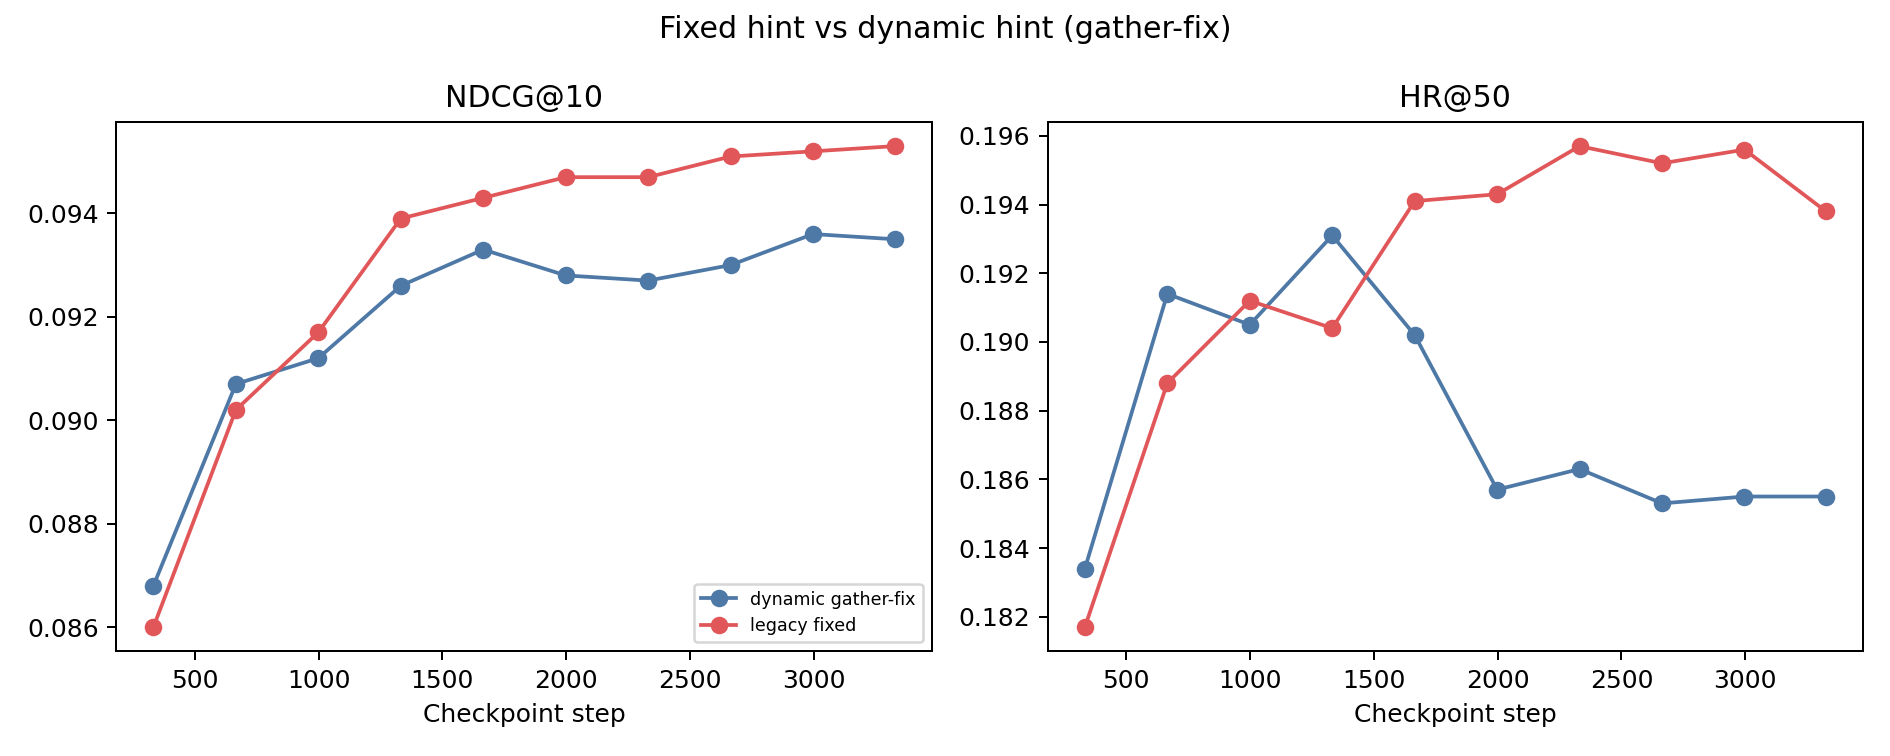
\includegraphics[width=\textwidth]{figures/dynamic_vs_fixed.png}
\caption{fixed hint 与 dynamic hint(gather-fix) 的逐 checkpoint 对比。}
\end{figure}
\footnotetext{来源：作者基于 \texttt{metrics\_inventory.csv} 对齐 checkpoint 后自绘。}

更细地看时间轨迹，会发现 dynamic 并不是从第一步就输 fixed。恰恰相反：
\begin{itemize}
\item 在 \texttt{checkpoint-333} 和 \texttt{666}，dynamic gather-fix 在 \texttt{NDCG@10} 上分别高 \texttt{0.0008} 和 \texttt{0.0005}。
\item 从 \texttt{checkpoint-999} 开始，fixed 反超并保持到结束。
\item 到后半程 \texttt{1998--3326}，fixed 对 dynamic 的优势大致稳定在 \texttt{NDCG@10 +0.0016--0.0021}、\texttt{HR@50 +0.0083--0.0101}。
\end{itemize}

这组形状非常像下面这个机制：
\begin{itemize}
\item dynamic 的 on-policy hint selection 在早期确实更贴合当前策略，所以起步略快；
\item 但 dynamic 的 stage gate 是 \texttt{rule\_hit\_any}。在当前 item-trie 下，完整正确 item 本质上只有一个，所以这个 gate 几乎等价于“那唯一正确 beam 这一步有没有刚好出现”；
\item 一旦这个 one-hit 事件在浅 stage 发生，dynamic 就直接锁定该 depth，并丢弃更深 stage 的候选；因此它优化的是“\textbf{最早撞中 1 条 beam 的深度}”，而不一定是“\textbf{最适合训练的深度}”；
\item hint depth 在线变化本身不是问题，问题是它现在对这个 one-hit 事件过于敏感：同一样本可能因为这一轮 16-beam 里是否冒出那一条 exact beam，而在 0/1/2/3 之间跳动；
\item fixed 虽然 map 可能陈旧，但在当前 \texttt{2 epoch + 1e-5} 的训练幅度下，stale-map drift 似乎没有这种 one-hit gate 带来的 depth 抖动更伤。
\end{itemize}

所以更准确的表述不是“dynamic 理论错了”，而是“\textbf{在当前训练强度下，策略漂移还不足以压过 one-hit gate 引入的 depth 抖动}”。这也解释了为什么 fixed 最终更强。

\subsection{sid-only 更直接对齐评测任务，但目前仍未优于 mixed-task}

这里需要修正我上一版报告里的一个判断。数据生成脚本 \texttt{preprocess\_data\_sft\_rl.py} 明确表明：
\begin{itemize}
\item 默认 mixed RL 训练集包含 \texttt{task1\_sid\_sft}、\texttt{task4\_hisTitle2sid}、\texttt{task5\_title\_desc2sid}。
\item 但 \texttt{rl\_valid}、\texttt{rl\_test} 只保留 \texttt{task1\_sid\_sft}。
\item \texttt{scripts/run\_instruments\_preprocess\_grec\_rl\_sid\_only.sh} 则通过 \texttt{RL\_ONLY\_TASK1=true} 只保留 task1 进入 RL 训练。
\end{itemize}

因此，你说得对：\texttt{sid-only} 训练确实\textbf{更直接对齐了最终评测任务}，不是我上一版写的那种“因为 benchmark 是 mixed-task 所以 sid-only 吃亏”。

即便如此，\texttt{dynamic hint sid-only} 的 best 点仍然弱于 mixed-task 的 \texttt{dynamic hint rule-only + gather fix}：
\begin{itemize}
\item \texttt{NDCG@10} 低 \texttt{0.0015}
\item \texttt{HR@10} 低 \texttt{0.0014}
\item \texttt{NDCG@50} 低 \texttt{0.0018}
\item \texttt{HR@50} 低 \texttt{0.0025}
\end{itemize}

这件事更合理的解释不是“sid-only 对错了 benchmark”，而是：
\begin{itemize}
\item task4 / task5 虽然不是最终评测任务，
\item 但它们和 task1 共享同一套 SID 目标空间，
\item 很可能在训练期提供了额外的 prefix routing / SID token semantics 监督。
\end{itemize}

因此，当前证据更像是在支持“\textbf{辅助任务带来了正迁移}”，而不是支持“mixed-task 只是因为口径更贴近评测”。不过这条仍然不是完美 apples-to-apples，因为 sid-only run 的 checkpoint 节奏与样本量都变了，所以最稳妥的后续工作仍然是做统一训练预算下的 paired rerun。

\subsection{ranking 没有显示出明确收益，而且有机制层面的解释}

当前最接近的实证对比是 dynamic hint 组：
\begin{itemize}
\item \texttt{dynamic hint + ranking}: \texttt{NDCG@10=0.0911}, \texttt{HR@50=0.1822}
\item \texttt{dynamic hint rule-only + gather fix}: \texttt{NDCG@10=0.0936}, \texttt{HR@50=0.1855}
\end{itemize}

排名 reward 版本在四个主指标上都更差。这里需要修正我上一版报告里的保守说法：\textbf{这条证据比“提示性证据”更强}。原因是 \texttt{ranking dynamic hint} 的 launcher 是 2026-03-28 才新增的，而 dynamic gather fix 本身在 2026-03-20 已经进入 trainer。也就是说，ranking dynamic 不是跑在“老 bug 版 dynamic”上的，它已经天然继承了 gather-fix 之后的 dynamic trainer。

即便如此，代码层也支持“ranking 不太对主矛盾”这个判断：当前 ranking reward 只在 group 里已经存在 exact hit 时，才会给 non-exact beams 一个 rank-based negative signal；对于 hardest case 的“整组都没有 exact hit”，ranking reward 直接归零。也就是说，它主要在“已经有成功样本的组里做 sharpening”，而不是在“完全没学会的组里提供更有用的梯度”。

\section{为什么 fixed 当前比 dynamic 更好}

\begin{figure}[H]
\centering
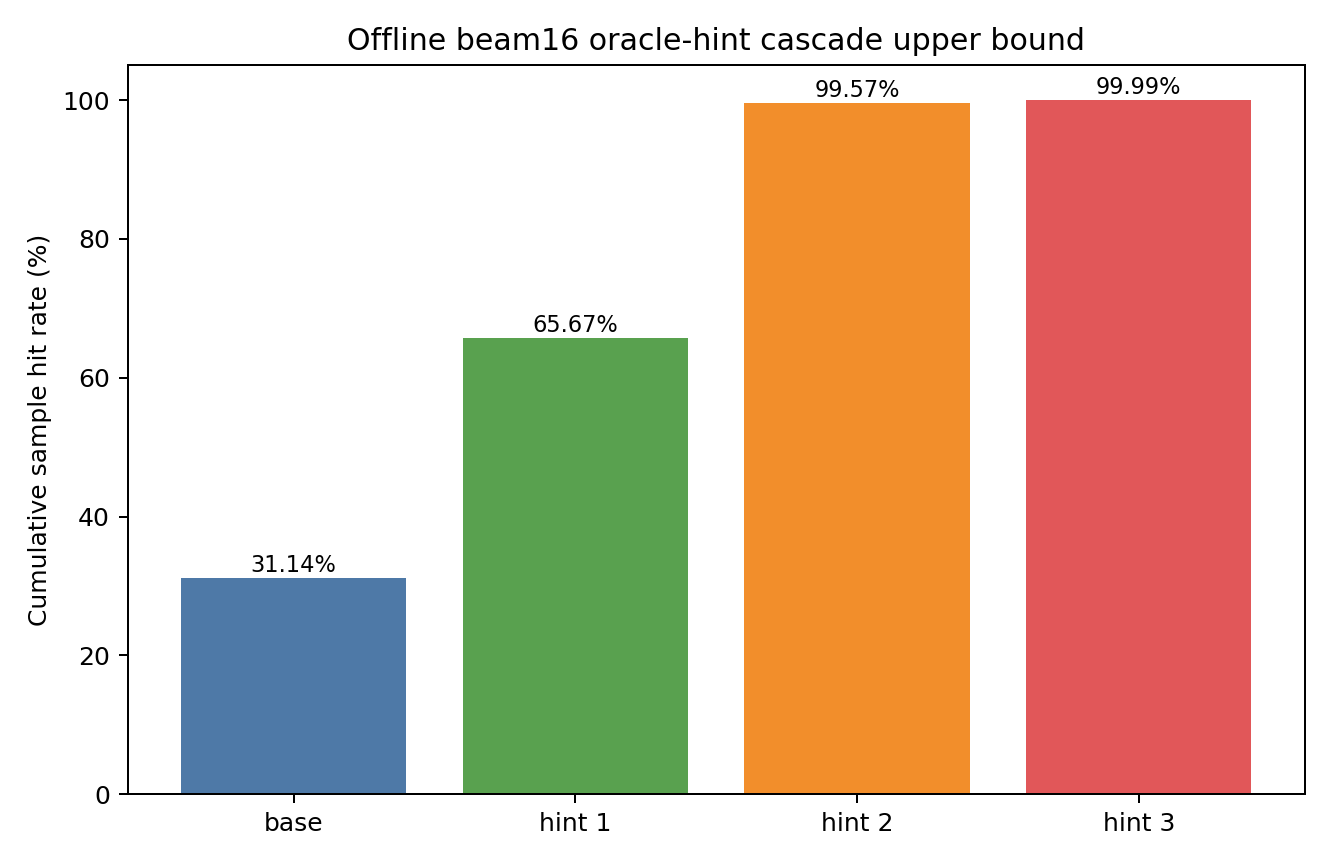
\includegraphics[width=0.8\textwidth]{figures/offline_stage_recovery.png}
\caption{离线 beam16 oracle-hint cascade 的 cumulative sample hit upper bound。}
\end{figure}
\footnotetext{来源：\texttt{temp/rl\_beam\_hint/instruments\_grec\_beam\_hint\_cascade\_20260314\_task\_index\_fix\_export\_summary.json}。}

\begin{figure}[H]
\centering
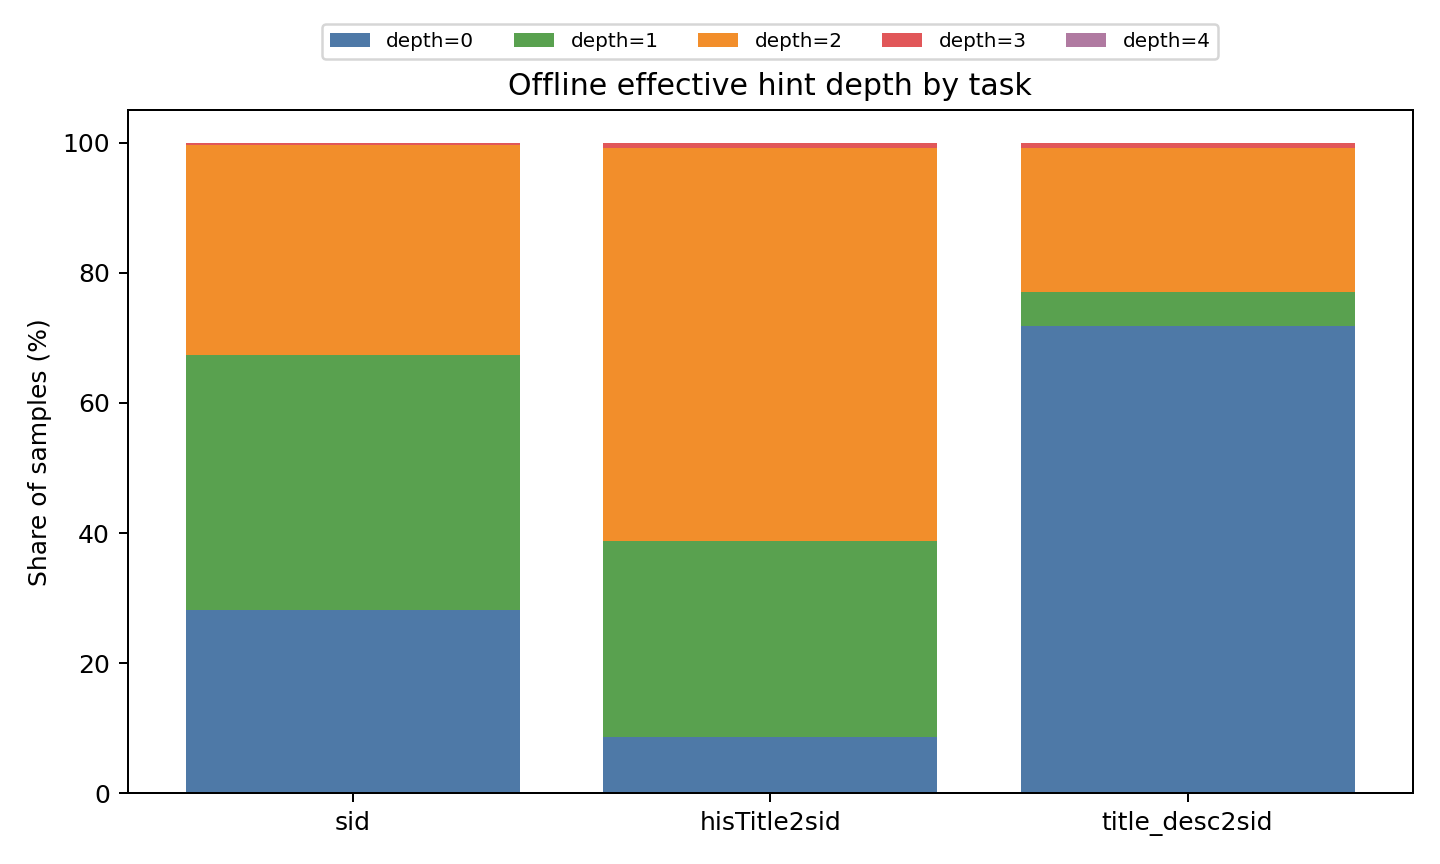
\includegraphics[width=0.84\textwidth]{figures/offline_task_depth_distribution.png}
\caption{离线 effective hint depth 的 task-level 分布。}
\end{figure}
\footnotetext{来源：\texttt{output/jupyter-notebook/genrec-hint-cascade-artifacts/instruments\_grec\_beam16\_hint\_difficulty\_table.csv}。}

\subsection{先把误解去掉：dynamic 的“变化”不是错，问题在于 gate 与优化目标不一致}

你指出得对，dynamic hint 的 hint depth 随当前策略变化，本来就是这个方法的定义，不应该被我上一版写成“变化本身有问题”。真正的问题不在“会变化”，而在于\textbf{现在 dynamic 用来决定 hint depth 的 gate，与后续真正被优化的 GRPO 信号不是同一个东西}：
\begin{itemize}
\item 代码里 dynamic stage 的停止条件是 \texttt{group\_rule\_hit\_any}；
\item 对每个 prompt group，只要当前 stage 的 16 条 beam 里有 \textbf{任意一条} exact hit，就直接选中这一 stage，后续更深的 stage 不再看；
\item 这意味着 dynamic 实际上选的是 \textbf{minimum-any-hit depth}。
\end{itemize}

但 pure \texttt{rule\_only} 下，GRPO 真正优化的是所选 stage 的\textbf{整组 reward / advantage 分布}。如果某个 stage 上 16 条 beam 里有 $k$ 条 exact hit，那么：
$$
r_i \in \{0,1\}, \qquad \bar r = \frac{k}{16}, \qquad A_i = r_i - \bar r
$$
\begin{itemize}
\item $r_i$：第 $i$ 条 beam 的 rule reward
\item $\bar r$：这一整个 prompt group 的平均 reward
\item $A_i$：进入 GRPO 的组内 centered advantage
\item $k$：这一 stage 上 exact-hit beam 的数量
\end{itemize}

所以 dynamic 当前更关键的问题不是“hint depth 会动”，而是：
\begin{itemize}
\item gate 只看 “$k>0$ 是否第一次成立”；
\item 但训练真正关心的是所选 stage 的整个 reward distribution，也就是 $k$ 到底有多大；
\item 如果浅 stage 只有 $k=1$，而更深 stage 会给 $k=4$、$k=8$ 甚至更多 exact-hit beams，dynamic 也完全看不到。
\end{itemize}

如果还沿用“variance”这个词，这里更准确指的是一种\textbf{非平滑的 prompt-schedule 跳变}：不是 beam search 本身随机，而是同一样本一旦在浅 stage 第一次让 $k$ 从 0 变成正数，dynamic 就会切到更浅的 conditioning。

\subsection{fixed 比 dynamic 强，不是因为 fixed 理论更对，而是因为当前 dynamic gate 太脆}

把 fixed 与 dynamic 放在一起看，更合理的解释是：
\begin{itemize}
\item fixed 提供的是一个\textbf{稳定但可能偏差}的 scaffold；
\item dynamic 提供的是一个\textbf{更自适应但 conditioning schedule 更不平滑}的 scaffold；
\item 在当前 \texttt{2 epoch + 1e-5} 的训练幅度下，稳定性收益似乎大于自适应收益。
\end{itemize}

这也解释了为什么 dynamic 在早期并不差，甚至略好，而后期被 fixed 反超：
\begin{itemize}
\item 早期模型很弱时，on-policy 动态 hint 确实更贴合当前能力，所以起步更快；
\item 但随着训练推进，dynamic 会越来越早地在浅 stage 触发 $k>0$，从而提前切到更浅的 prompt conditioning；
\item 这使 dynamic 更像是在优化“当前策略最小需要几层 hint 才能至少打中 1 条 beam”，而不是优化“哪个 hint depth 最利于形成稳定、可迁移的训练分布”。
\end{itemize}

换句话说，dynamic 现在选的是 \textbf{minimum hit depth}，而不是真正意义上的 \textbf{best training depth}。这两者并不等价。

\subsection{为什么错版 fixed 反而更好：少一些 hint 可能更接近最终目标，但前提是要稳定}

旧的 index-only bug 给 hardest task 大幅少给了 hint，但它仍然是\textbf{稳定地少给}，不是像 dynamic 那样随 step 抖动。这个现象更像是在无意中做了一种“浅 scaffold curriculum”：
\begin{itemize}
\item 比正确 task+index map 更少的 hint，使训练分布更接近最终无 hint 评测；
\item 但因为这个浅 hint 是离线固定的，所以不会像 dynamic 那样受 one-hit 门控影响来回跳。
\end{itemize}

因此，当前最合理的理解不是“dynamic 本该更好却失败了”，而是：
\begin{itemize}
\item \textbf{hint 少一点} 可能对 no-hint transfer 有好处；
\item \textbf{hint 深度稳定} 也有明显好处；
\item 旧 fixed 恰好踩中了“更浅但更稳”这个组合；
\item 修复后的 fixed 变得“更准但更深”，dynamic 则是“可能更浅但不够稳”。
\end{itemize}

这三者的 trade-off，刚好能解释当前排序：旧 fixed 最强，taskfix fixed 次之，dynamic gather-fix 再后。

\subsection{如果要让 dynamic 真正赢 fixed，它需要改 stopping signal，而不是只靠在线变化}

基于现在的代码，我认为 dynamic 要真正超过 fixed，至少要改掉现在这个 \texttt{rule\_hit\_any} gate。更合理的候选包括：
\begin{itemize}
\item 不再用“是否出现 1 条 exact hit”作为 stopping 条件，而用 \texttt{rule\_hit\_count}、\texttt{group mean reward}、\texttt{mean prefix progress} 或 top-k beam 质量。
\item 把 dynamic depth 和一个离线 teacher map 混合，而不是完全由当步 rollout 决定。
\item 对同一样本引入 depth hysteresis/EMA，避免 0/1/2/3 之间来回抖动。
\end{itemize}

也就是说，dynamic 的问题不是“它会变”，而是“\textbf{它现在用错了 gate}”。

\section{代码层解释：为什么 ranking 不明显、为什么 prefix shaping 容易不稳定}

\subsection{ranking reward 对 hardest case 几乎没有帮助}

\texttt{rewards/ranking\_reward.py} 的 reward setup 本质上是：

\begin{lstlisting}[caption={当前 reward mode 分支的核心定义},label={lst:reward-setup}]
if mode == "rule_only":
    return [rule_reward], None
if mode == "prefix_only":
    return _append_rule_reward_probe([prefix_func, ndcg_func], None)
if mode == "ranking":
    return [rule_reward, get_ndcg_rule_reward(num_beams)], None
\end{lstlisting}

而 \texttt{ndcg\_rule\_reward} 的行为不是“prefix 越长越奖励”，而是“\textbf{当组内已有 exact hit 时，对 non-exact beams 按 rank 给负信号}”。更关键的是，GRPO 最终优化的不是原始 reward，而是组内 advantage：

\begin{lstlisting}[caption={当前 dynamic/fixed trainer 与普通 GRPO 一样，最终用组内 centered advantage},label={lst:advantage}]
rewards = (rewards_per_func * self.reward_weights.to(device).unsqueeze(0)).nansum(dim=1)
mean_grouped_rewards = rewards.view(-1, self.num_generations).mean(dim=1)
mean_grouped_rewards = mean_grouped_rewards.repeat_interleave(self.num_generations, dim=0)
advantages = rewards - mean_grouped_rewards
\end{lstlisting}

所以 ranking 在这里的作用实际上更弱：
\begin{itemize}
\item 对完全没解开的 group，ranking reward 直接没有额外帮助；
\item 对已经有 exact hit 的 group，它主要只是\textbf{重新排列这一组 rollout 之间的相对次序}；
\item 它并不增加正样本数量，也不解决 zero-hit group 没梯度的问题；
\item 在 current setup 下，它本质上更像“rollout 内部排序信号”，而不是能改变样本级可学性的主信号。
\end{itemize}

这与离线 bundle 的难度画像正好冲突：当前 hardest case 主要集中在前两位 SID token 的 routing 问题，而不是“已经有 exact hit 后，怎样把 beam rank 排得更尖”。

\subsection{prefix shaping 的问题不在“粒度”，而在“credit assignment”}

\texttt{token\_prefix\_grpo\_trainer.py} 里，matched prefix token 默认得到的是 \texttt{1/L} 级别的局部正信号；如果采用 \texttt{token\_adv\_total\_token\_normalize}，则会把 prefix token reward 与 NDCG token reward 先合成，再按 token 位置做 group normalization。代码本身已经说明了这个设计非常敏感：
\begin{itemize}
\item raw token-level 组合会把不同 token 位置、不同 rollout 的信号直接混在一起；
\item totalnorm 至少让这些信号在同一 token-wise normalization 语义下比较；
\item errtok 再进一步改变了负信号的覆盖范围，但当前实验没有显示出收益。
\end{itemize}

所以这条线当前最好的表述不是“我们已经找到最优 token reward”，而是“\textbf{我们证明了 token-level prefix shaping 能否成立，主要取决于 normalization 细节；没有正确 normalization，会直接崩}”。

\section{我们现在最可信的 contribution 是什么}

\begin{findingbox}{可以写进论文的三点 contribution}
\begin{itemize}
\item \textbf{Contribution 1: task-aware offline hint analysis 识别了 GenRec semantic-ID RL 的主瓶颈。} 离线 beam16 cascade 显示，大多数样本的主要困难集中在前两位 SID token；不同 task 的难度形状明显不同，不能被单一局部树结构完全解释。
\item \textbf{Contribution 2: oracle scaffold 比复杂 reward shaping 更有效。} 现有实验表明，fixed hint 能以几乎不损失 top-10 的代价，显著修复 plain rule-only 的 coverage 损失；这比当前任何单纯改 reward 形状的方案都更稳定、更有故事性。
\item \textbf{Contribution 3: 我们把“稀疏 reward 的问题”重新定位成“可迁移 scaffold 学习的问题”。} 离线上界几乎 100\% 可解，但 no-hint 在线评测仍有明显 gap；这说明真正要解决的不是简单地换 dense reward，而是如何把 offline scaffold upper bound 转移成 test-time 无 hint 能力。
\end{itemize}
\end{findingbox}

如果现在就要为论文定主线，我会建议主叙事是：
\begin{itemize}
\item 先用离线 hint bundle 证明 \textbf{semantic-ID recommendation 的 hardest routing 集中在 prefix}；
\item 再用 RL ablation 证明 \textbf{复杂 reward shaping 并不稳定，oracle scaffold 更有效}；
\item 最后把 fixed hint 看成第一版可行系统，把 future work 指向“如何把 oracle scaffold 逐步蒸馏成无 hint policy”。
\end{itemize}

\section{后续应该怎么做}

\subsection{优先级最高：把 fixed hint 变成真正的主线方法}

最值得继续加资源的不是再开更多 prefix reward 变体，而是 fixed hint 主线，具体建议：
\begin{itemize}
\item 以 \texttt{taskfix-b16} 作为更可信的工程基线继续长训和复现。
\item 单独做 \texttt{fixed hint apply to eval = true/false} 的 paired evaluation，用于拆出“hinted test-time upper bound”和“no-hint transfer gain”。
\item 增加一条 \textbf{hint dropout / hint annealing} 线，验证能否把训练期 scaffold 更好地蒸馏回无 hint 测试表现。
\end{itemize}

\subsection{第二优先级：把 dynamic hint 变成 scheduler ablation，而不是主结果}

dynamic hint 目前最合理的定位不是主方法，而是：
\begin{itemize}
\item 证明 online scheduler 方向有价值；
\item 提供对 fixed hint map 的 online 近似；
\item 为后续 adaptive scaffold policy 提供原型。
\end{itemize}

但在它真正成为主结果之前，至少要补两件事：
\begin{itemize}
\item 把 dynamic 的 stopping criterion 从 \texttt{rule\_hit\_any} 升级成更稳的质量统计，再看它是否还能输给 fixed；
\item 用与 \texttt{rule-only dynamic hint} 完全对齐的 seed / 训练预算 / 保存节奏，再做一次 \texttt{ranking dynamic hint} 配对复现，确认当前劣势不是偶然种子；
\item 统一 mixed-task 与 sid-only 的训练步数、checkpoint 采样节奏，再做更干净的 task ablation。
\end{itemize}

\subsection{第三优先级：reward 线只保留最必要的四条}

当前 reward 线已经足以收敛，不需要继续大规模铺开：
\begin{itemize}
\item \texttt{rule-only rerun}
\item baseline mixed GRPO
\item \texttt{prefix tokenadv totalnorm}
\item fixed hint taskfix
\end{itemize}

这四条已经能覆盖：
\begin{itemize}
\item 稀疏 exact reward baseline
\item mixed reward baseline
\item “reward shaping 能否救回来”的最好版本
\item “scaffold 是否比 shaping 更有效”的最强证据
\end{itemize}

\subsection{任务设计层面：不要过早只押 sid-only，要先做 clean ablation}

从离线 bundle 和 sid-only run 的结果一起看，更合理的方向是：
\begin{itemize}
\item 不要先验地断定 sid-only 一定更好或 mixed-task 一定更好；
\item 在统一训练预算下，把 sid-only 与 mixed-task 做真正配对实验；
\item 明确引入 task-aware scaffold depth、task-aware sampling 或 task-aware curriculum；
\item 如果要做更细的 RL objective，先按 task 观察哪一类样本主要失败在第几层 SID token，再决定是否需要不同 reward/hint policy。
\end{itemize}

\section{结论与后续问题}

\subsection{已经被强支持的结论}

\begin{itemize}
\item fixed hint 是当前最值得继续推进的主线方法，它几乎保住了 best top-10，同时显著修复了 rule-only 的 coverage 损失。
\item 复杂 reward shaping 目前没有展示出超越 scaffold 的稳定收益；其中 totalnorm 是 token-level shaping 可用的必要条件之一。
\item dynamic 当前输给 fixed，更像是输在 \texttt{rule\_hit\_any} 这种 one-hit gate 带来的 depth 抖动，而不是输在“在线自适应”这个想法本身。
\item 虽然评测任务是 task1-only，但 mixed-task 训练目前仍略优于 sid-only，说明 task4/task5 可能带来了正的辅助迁移。
\end{itemize}

\subsection{较大概率为真，但还需要补 cleaner ablation 的结论}

\begin{itemize}
\item ranking reward 在当前任务里很可能不是主矛盾，至少现有结果没有显示收益。
\item task-aware fixed hint map 的小幅 top-10 回落更像“修复 index collision 后，hint 变深带来的 transfer 代价”，而不是方法本身无效。
\item dynamic hint 的最终潜力还没被跑干净，但它更像 scheduler/teacher，而不是当前最强成品方法。
\end{itemize}

\subsection{仍然未知、值得马上验证的问题}

\begin{itemize}
\item fixed hint 的收益里，有多少来自 train-time scaffold 本身，有多少可以转化成 no-hint inference gain？
\item hint dropout、hint annealing 或 teacher-student distillation 能否把 fixed hint 的 coverage 优势更多转化成无 hint 的 top-10 改善？
\item ranking reward 若结合 prefix progress，而不是只在 exact-hit group 内做 rank penalty，是否会更贴近真实瓶颈？
\end{itemize}

\appendix

\section{用户指定目录的分类索引}

\begin{longtable}{p{4.0cm}p{3.3cm}p{2.2cm}p{1.6cm}p{1.5cm}}
\toprule
Label & Classification & Best ckpt & Best NDCG@10 & Best HR@50 \\
\midrule
\endhead
Dynamic hint + ranking & main\_hint & checkpoint-1665 & 0.0911 & 0.1822 \\
Dynamic hint rule-only (old) & main\_hint\_superseded\_by\_gather\_fix & checkpoint-1665 & 0.0919 & 0.1905 \\
Dynamic hint rule-only + gather fix & main\_hint & checkpoint-2997 & 0.0936 & 0.1855 \\
Dynamic hint sid-only & main\_hint & checkpoint-2394 & 0.0921 & 0.1830 \\
Fixed hint mixed-single & main\_hint & checkpoint-3326 & 0.0953 & 0.1938 \\
Fixed hint task+index early & early\_taskfix\_run & checkpoint-666 & 0.0894 & 0.1864 \\
Fixed hint taskfix b16 & main\_hint & checkpoint-2997 & 0.0931 & 0.1941 \\
Prefix old alias & legacy\_alias & checkpoint-1665 & 0.0863 & 0.1631 \\
Prefix backup & partial\_backup & checkpoint-333 & 0.0815 & 0.1608 \\
Prefix seq only broken run & superseded\_broken\_run & checkpoint-1332 & 0.0389 & 0.1023 \\
Rule only old run & superseded\_old\_run & checkpoint-333 & 0.0761 & 0.1494 \\
Baseline mixed GRPO & main\_reward & checkpoint-1665 & 0.0952 & 0.1696 \\
Rule only rerun & main\_reward & checkpoint-2997 & 0.0960 & 0.1681 \\
Prefix only & main\_reward & checkpoint-1332 & 0.0862 & 0.1612 \\
Prefix seq only rerun & main\_reward & checkpoint-1332 & 0.0857 & 0.1636 \\
Prefix token only & main\_reward & checkpoint-1665 & 0.0815 & 0.1668 \\
Prefix tokenadv raw & main\_reward & checkpoint-999 & 0.0476 & 0.0991 \\
Prefix tokenadv totalnorm & main\_reward & checkpoint-3326 & 0.0906 & 0.1809 \\
Prefix tokenadv errtok & main\_reward & checkpoint-999 & 0.0796 & 0.1513 \\
Prefix backup single checkpoint & single\_checkpoint\_backup & checkpoint-333 & 0.0815 & 0.1608 \\
\bottomrule
\end{longtable}

\section{Legacy / Superseded Run 结果表}

\begin{table}[H]
\centering
\small
\begin{tabular}{p{4.2cm}p{1.7cm}cccc}
\toprule
Variant & Best ckpt & NDCG@10 & HR@10 & NDCG@50 & HR@50 \\
\midrule
Prefix old alias & checkpoint-1665 & 0.0863 & 0.1060 & 0.0985 & 0.1631 \\
Prefix backup & checkpoint-333 & 0.0815 & 0.0998 & 0.0946 & 0.1608 \\
Prefix seq only broken run & checkpoint-1332 & 0.0389 & 0.0494 & 0.0504 & 0.1023 \\
Rule only old run & checkpoint-333 & 0.0761 & 0.0907 & 0.0885 & 0.1494 \\
\bottomrule
\end{tabular}
\caption{legacy / superseded run 只用于解释历史演化和 bug 修复，不作为主结论。}
\end{table}

\section{来源清单}

\scriptsize
\begin{longtable}{p{1cm}p{1.3cm}p{4.0cm}p{8.0cm}}
\toprule
ID & 模态 & 标题 & 路径 \\
\midrule
\endhead
S1 & data & Checkpoint metrics inventory & \texttt{/Users/fanghaotian/Desktop/src/GenRec/docs/deepresearch/genrec\_rl\_study\_2026-03-28/data/metrics\_inventory.csv} \\
S2 & data & Beam16 hint difficulty table & \texttt{/Users/fanghaotian/Desktop/src/GenRec/output/jupyter-notebook/genrec-hint-cascade-artifacts/instruments\_grec\_beam16\_hint\_difficulty\_table.csv} \\
S3 & data & Beam16 cascade summary & \texttt{/Users/fanghaotian/Desktop/src/GenRec/temp/rl\_beam\_hint/instruments\_grec\_beam\_hint\_cascade\_20260314\_task\_index\_fix\_export\_summary.json} \\
S4 & data & Task-aware fixed hint map & \texttt{/Users/fanghaotian/Desktop/src/GenRec/output/jupyter-notebook/genrec-hint-cascade-artifacts/instruments\_grec\_beam16\_task\_index\_fix\_hint\_map.json} \\
S5 & code & Reward setup implementation & \texttt{/Users/fanghaotian/Desktop/src/GenRec/rewards/ranking\_reward.py} \\
S6 & code & Token-level prefix trainer & \texttt{/Users/fanghaotian/Desktop/src/GenRec/token\_prefix\_grpo\_trainer.py} \\
S7 & code & Main RL trainer entrypoint & \texttt{/Users/fanghaotian/Desktop/src/GenRec/trl\_trainer.py} \\
S8 & code & Dynamic/fixed hint trainer internals & \texttt{/Users/fanghaotian/Desktop/src/GenRec/fixed\_hint\_grpo\_trainer.py} \\
S9 & code & External evaluation pipeline & \texttt{/Users/fanghaotian/Desktop/src/GenRec/evaluate.py} \\
S10 & doc & Main results weekly report & \texttt{/Users/fanghaotian/Desktop/src/GenRec/docs/genrec\_main\_results\_weekly\_2026-03-18.zh.md} \\
S11 & doc & Reward form analysis & \texttt{/Users/fanghaotian/Desktop/src/GenRec/docs/genrec\_rl\_reward\_forms\_2026-03-13.md} \\
S12 & doc & Dynamic vs fixed hint implementation note & \texttt{/Users/fanghaotian/Desktop/src/GenRec/docs/genrec\_dynamic\_fixed\_hint\_metrics\_2026-03-17.zh.md} \\
\bottomrule
\end{longtable}

\end{document}
